\section{Auswertung}
\label{sec:Auswertung}
Im Folgenden wird der Fehler von Größen gebildet, die von mehreren fehlerbehafteten Größen abhängig sind. Dieser Fehler wird mithilfe der Gaußschen 
Fehlerfortpflanzung 
$$\Delta f = \sqrt{\sum_{i = 1}^{n} \left( \frac{\partial f}{\partial x_i} \right)^2 \cdot \left(\Delta x_i \right)^2}$$
bestimmt. Dabei bezeichnet $n$ die Anzahl der Größen, von denen $f$ abhänig ist, $x_i$ die jeweilige Größe und $\Delta x_i$ den Fehler dieser. \\

  \subsection{Verdampfungswärme von Wasser bis 1 bar}
   Der zu Anfang gemessene Umgebungsdruck $p_0$ beträgt $985\,\unit{\milli\bar}$ bei einer Umgebungstemperatur von $22 \,\unit{\celsius}$. 
  Die gemessenen Werte für das Druckverhalten bei ansteigendender Temperatur für 
  Druck unter 1 bar ist in Tabelle (\ref{tab:Druck_unter_1_bar}) aufgelistet. Diese Werte werden in Abbildung (\ref{fig:Druck_unter_1_bar}) aufgetragen.  

    \begin{longtblr}[
      caption = {Gemessener Druck $p$ bei verschiedenen Temperaturen $T$},
      label = {tab:Druck_unter_1_bar},
      ]{
      colspec = {c c c c c c},
       }
      \toprule
      $T \, \left[\unit{\celsius}\right]$ & $p \, \left[\unit{\milli\bar}\right]$ & $T \, \left[\unit{\celsius}\right]$ & $p \, \left[\unit{\milli\bar}\right]$ & $T \, \left[\unit{\celsius}\right]$ & $p \, \left[\unit{\milli\bar}\right]$\\ 
    \midrule
      $25 \pm 1$ & $95 \pm 1$  & $51 \pm 1$ & $197 \pm 1$ & $77 \pm 1$ & $438 \pm 1$ \\                     
      $26 \pm 1$ & $98 \pm 1$  & $52 \pm 1$ & $202 \pm 1$ & $78 \pm 1$ & $453 \pm 1$ \\                               
      $27 \pm 1$ & $102 \pm 1$  & $53 \pm 1$ & $207 \pm 1$ & $79 \pm 1$ & $471 \pm 1$ \\                   
      $28 \pm 1$ & $105 \pm 1$  & $54 \pm 1$ & $212 \pm 1$ & $80 \pm 1$ & $487 \pm 1$ \\                   
      $29 \pm 1$ & $108 \pm 1$  & $55 \pm 1$ & $218 \pm 1$ & $81 \pm 1$ & $507 \pm 1$ \\                  
      $30 \pm 1$ & $112 \pm 1$  & $56 \pm 1$ & $225 \pm 1$ & $82 \pm 1$ & $528 \pm 1$ \\                   
      $31 \pm 1$ & $116 \pm 1$  & $57 \pm 1$ & $231 \pm 1$ & $83 \pm 1$ & $547 \pm 1$ \\                   
      $32 \pm 1$ & $119 \pm 1$  & $58 \pm 1$ & $237 \pm 1$ & $84 \pm 1$ & $578 \pm 1$ \\                   
      $33 \pm 1$ & $122 \pm 1$  & $59 \pm 1$ & $245 \pm 1$ & $85 \pm 1$ & $592 \pm 1$ \\                   
      $34 \pm 1$ & $126 \pm 1$  & $60 \pm 1$ & $252 \pm 1$ & $86 \pm 1$ & $612 \pm 1$ \\                   
      $35 \pm 1$ & $131 \pm 1$  & $61 \pm 1$ & $258 \pm 1$ & $87 \pm 1$ & $635 \pm 1$ \\                   
      $36 \pm 1$ & $134 \pm 1$  & $62 \pm 1$ & $265 \pm 1$ & $88 \pm 1$ & $656 \pm 1$ \\                   
      $37 \pm 1$ & $138 \pm 1$  & $63 \pm 1$ & $273 \pm 1$ & $89 \pm 1$ & $678 \pm 1$ \\                   
      $38 \pm 1$ & $141 \pm 1$  & $64 \pm 1$ & $281 \pm 1$ & $90 \pm 1$ & $700 \pm 1$ \\                   
      $39 \pm 1$ & $145 \pm 1$  & $65 \pm 1$ & $290 \pm 1$ & $91 \pm 1$ & $724 \pm 1$ \\                   
      $40 \pm 1$ & $149 \pm 1$  & $66 \pm 1$ & $299 \pm 1$ & $92 \pm 1$ & $753 \pm 1$ \\                  
      $41 \pm 1$ & $153 \pm 1$  & $67 \pm 1$ & $308 \pm 1$ & $93 \pm 1$ & $775 \pm 1$ \\                   
      $42 \pm 1$ & $157 \pm 1$  & $68 \pm 1$ & $317 \pm 1$ & $94 \pm 1$ & $809 \pm 1$ \\                   
      $43 \pm 1$ & $162 \pm 1$  & $69 \pm 1$ & $327 \pm 1$ & $95 \pm 1$ & $835 \pm 1$ \\                   
      $44 \pm 1$ & $166 \pm 1$  & $70 \pm 1$ & $337 \pm 1$ & $96 \pm 1$ & $867 \pm 1$ \\                   
      $45 \pm 1$ & $170 \pm 1$  & $71 \pm 1$ & $348 \pm 1$ & $97 \pm 1$ & $899 \pm 1$ \\                    
      $46 \pm 1$ & $174 \pm 1$  & $72 \pm 1$ & $360 \pm 1$ & $98 \pm 1$ & $938 \pm 1$ \\                   
      $47 \pm 1$ & $178 \pm 1$  & $73 \pm 1$ & $373 \pm 1$ & $99 \pm 1$ & $989 \pm 1$ \\                   
      $48 \pm 1$ & $183 \pm 1$  & $74 \pm 1$ & $387 \pm 1$ & $100 \pm 1$ & $999 \pm 1$ \\                   
      $49 \pm 1$ & $187 \pm 1$  & $75 \pm 1$ & $401 \pm 1$ & & \\ 
      $50 \pm 1$ & $192 \pm 1$  & $76 \pm 1$ & $417 \pm 1$ & & \\ 
      \bottomrule
    \end{longtblr}
     
     %Der Druck als $\ln{\frac{p}{p_0}}$ auf der y Achse und die Temperatur in $\frac{1}{T} \,\left[\frac{1}{\symup{K}}\right]$ auf der x-Achse. 


    \begin{figure}[H]
      \centering
      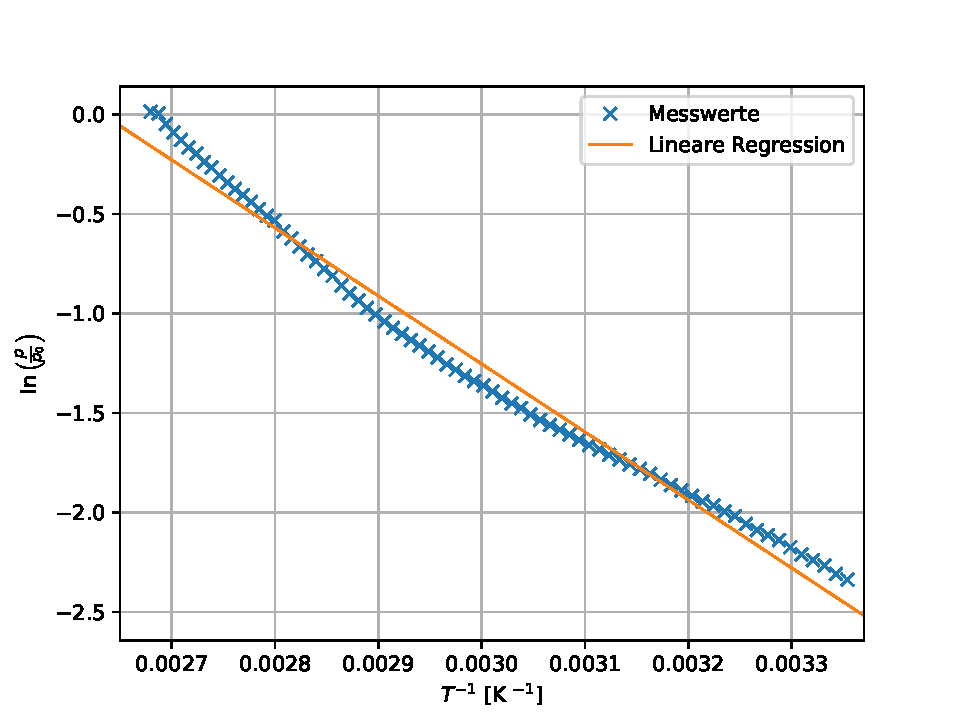
\includegraphics[width=0.977\linewidth]{plot1.pdf}
      \caption{Graphische Darstellung der Messwerte aus Tabelle (\ref{tab:Druck_unter_1_bar}) mit Ausgleichsgerade.}
      \label{fig:Druck_unter_1_bar}
    \end{figure}
    Die Ausgleichsgerade hat die Form 

    \begin{equation}
      \label{eqn:Ausgleichsgerade}
      \ln{\left(\frac{p}{p_0}\right)} = m \cdot \frac{1}{T} + n \, . 
    \end{equation}

    Für $m$ und $n$ ergeben sich die Werte $m = (-3417 \pm 53) \, \unit{\kelvin}$
    und $n = (9,0 \pm 0,2)$.
    Da $p$ unter 1 bar ist, dürfen die Vereinfachungen angenommen werden, die zu Gleichung (\ref{eqn:Druck_p}) führen. Diese Formel umgestellt ist 
    \begin{equation}
      \label{eqn:Druck_p_umgestellt}
      \ln{\left(\frac{p}{p_0}\right)} = - \frac{L}{R} \cdot \frac{1}{T} \, . 
    \end{equation}
    Mithilfe der Ausgleichsgerade (\ref{eqn:Ausgleichsgerade}) wird Formel 
    (\ref{eqn:Druck_p_umgestellt}) nach 
    \begin{align}
      m &= - \frac{L}{R} \\
      \Leftrightarrow L &= - \, m \cdot R
    \end{align}
    umgestellt. Für $R = 8,3145 \, \unit[per-mode=reciprocal]{\joule\per\mol\per\kelvin}$ \cite{R_Konstante} ergibt dies einen Wert von $L = (28,4 \pm 0,4) \cdot 10^3 \, \unit[per-mode=reciprocal]{\joule\per\mol}$.
    \\
    Zur Berechnung der inneren Verdampfungswärme $L_{\text{i}}$ wird Formel (\ref{eqn:Verdampfungswaerme}) verwendet. Diese umgestellt ergibt 
    \begin{equation}
      L_{\text{i}} = L - L_{\text{a}} \, . 
    \end{equation}
    Die äußere Verdampfungswärme $L_{\text{a}}$ wird mithilfe der ideale Gasgleichung (\ref{eqn:idealeGasgleichung}) für eine Temperatur $T_{\text{a}}$ von $373 \, \unit{\kelvin}$ wie folgt abgeschätzt
    \begin{equation}
      L_{\text{a}} = R \cdot  T_{\text{a}}\, . 
    \end{equation}
    Dies ergibt $L_{\text{a}} = 3,1013 \cdot 10³ \, \unit[per-mode=reciprocal]{\joule\per\mol}$. 
    Mithilfe von $L_{\text{a}}$ wird $L_{\text{i}} = (25,3 \pm 0,4) \cdot 10³ \, \unit[per-mode=reciprocal]{\joule\per\mol}$ bestimmt. 
    Um die Einheit der Energie $L_{\text{i}}$ in eine Energie mit Einheit Elektronenvolt pro Molekül $L_{\text{i,M}}$ umzurechnen, wird 
    \begin{equation}
      L_{\text{i,M}} = \frac{L_{\text{i}}}{\symup{N} \cdot \symup{e}}
      \label{eqn:L_Molekül}
    \end{equation}
    angewandt. $\symup{N}$ ist dabei die Avogadrokonstante $6,0221 \cdot 10^{23} \, \symup{mol^{-1}}$ \cite{N_Konstante} und $\symup{e}$ die Elementarladung mit 
    $\symup{e} = 1,6022 \cdot 10^{-19} \, \unit{\ampere\second}$ \cite{e_Konstante}. 
    Durch Gleichung (\ref{eqn:L_Molekül}) wird $L_{\text{i,M}}$ berechnet zu $L_{\text{i,M}} = (0,262 \pm 0,005) \, \symup{e}\symup{V}$.
    
    \subsection{Verdampfungswärme von Wasser von 1 bar bis 15 bar}
    Im Folgenden werden alle Variablen, die zu diesem Experiment gehören, mit Index $2$ versehen, da dies das 2. Teilexperiment ist.
    Da der Druck des Wasserdampfes und damit auch die betrachtete Temperatur 
    nun deutlich höher ist, wird $L_2$ nicht mehr als Konstante angenommen werden.
    Zur Berechnung wird die Clausius-Clapeyronsche Gleichung (\ref{eqn:ClausiusClapeyronscheGleichung}) 
    verwendet. Die umgestellte Form dieser Gleichung ist
    \begin{equation}
      L_2 = T_2 \cdot (V_{\text{D,2}} - V_{\text{F,2}}) \cdot \frac{\symup{d}p_2}{\symup{d}T_2} \, .
      \label{eqn:L_neue_Form}
    \end{equation}
    
    Zur Bestimmung von $L_2$ wird demnach die Ableitung der Druckkurve nach $T_2$ benötigt. 
    Ein Ausdruck für $p_2$ wird im Folgenden durch das Auswerten der Messwerte, die in Tabelle (\ref{tab:Druck_ueber_1_bar}) aufgeführt sind, 
    berechnet. 

    \begin{table}[H]
      \centering
      \caption{Gemessene Temperaturen $T_2$ bei verschiedenen Drucken $p_2$}
      \label{tab:Druck_ueber_1_bar}
      \begin{tblr}{colspec={c c}}
          \toprule
          $p_2 \left[\symup{bar}\right]$ & $T_2 \left[\unit{\celsius}\right]$ \\
          \midrule
          $1 \pm 0,5$ & $116 \pm 1$ \\
          $2 \pm 0,5$ & $132 \pm 1$ \\
          $3 \pm 0,5$ & $141 \pm 1$ \\
          $4 \pm 0,5$ & $150 \pm 1$ \\
          $5 \pm 0,5$ & $156 \pm 1$ \\
          $6 \pm 0,5$ & $162 \pm 1$ \\
          $7 \pm 0,5$ & $168 \pm 1$ \\
          $8 \pm 0,5$ & $173 \pm 1$ \\
          $9 \pm 0,5$ & $176 \pm 1$ \\
          $10 \pm 0,5$ & $181 \pm 1$ \\
          $11 \pm 0,5$ & $185 \pm 1$ \\
          $12 \pm 0,5$ & $189 \pm 1$ \\
          $13 \pm 0,5$ & $192 \pm 1$ \\
          $14 \pm 0,5$ & $195 \pm 1$ \\
          $15 \pm 0,5$ & $198 \pm 1$ \\
          \bottomrule
      \end{tblr}
    \end{table}
    
    Diese Messwerte werden in Abbildung (\ref{fig:Druck_ueber_1_bar}) mit einem Ausgleichspolynom 3. Grades dargestellt.
    Dieses hat die Form 
    \begin{equation}
      p_2 = a \cdot T_2³ + b \cdot T_2² + c \cdot T_2 + d \,.
    \end{equation}
    Die benötigte Ableitung nach $T_2$ hat demnach die Form
    \begin{equation}
      \frac{\symup{d}p_2}{\symup{d}T_2} = 3  a \cdot T_2² + 2 b \cdot T_2 + c \,.
    \end{equation}
    Die Berechnung der Parameter ergibt 
    \begin{align*}
      a &= (0,00064 \pm 0,00021) \, \unit[per-mode=fraction]{\kilo\pascal\per\kelvin\tothe{3}} \\
      b &= (-0.66 \pm 0.27)\, \unit[per-mode=fraction]{\kilo\pascal\per\kelvin\tothe{2}} \\
      c &= (227 \pm 117) \, \unit[per-mode=fraction]{\kilo\pascal\per\kelvin} \\
      d &= (-26160 \pm 16842) \, \unit{\kilo\pascal} \, .
    \end{align*}

    \begin{figure}[H]
      \centering
      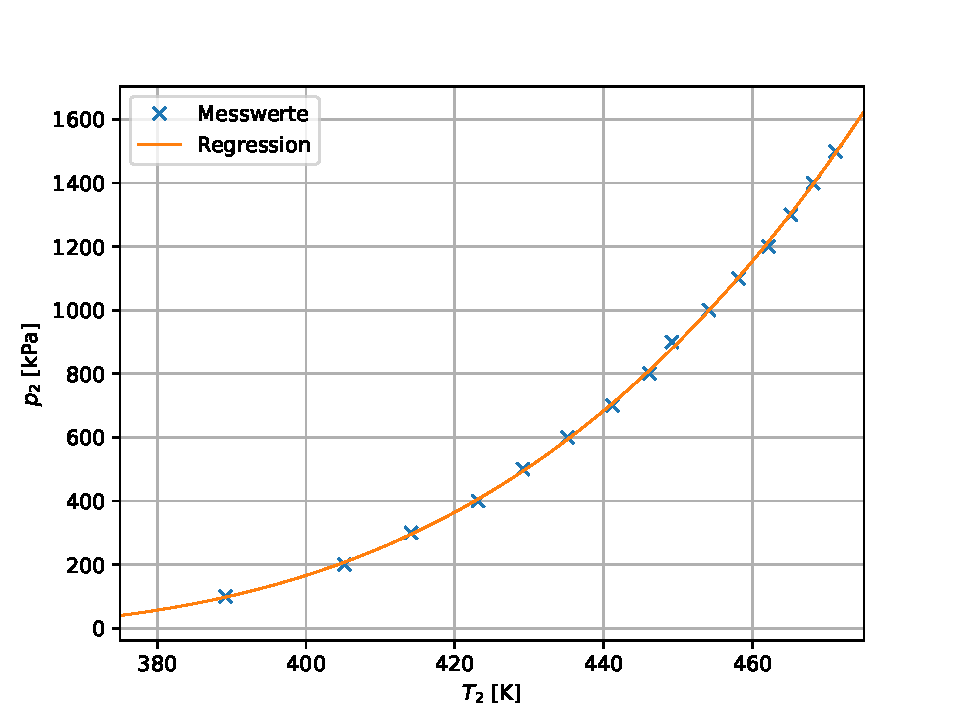
\includegraphics{plot2.pdf}
      \caption{Graphische Darstellung der Messwerte aus Tabelle (\ref{tab:Druck_ueber_1_bar}) mit Ausgleichspolynom 3. Grades.}
      \label{fig:Druck_ueber_1_bar}
    \end{figure}
    
    $V_{\text{D,2}}$ wird in dieser Rechnung nicht durch die ideale Gasgleichung ausgedrückt, da der Druck für diese
    Annahme zu hoch ist. Die nun verwendete Näherung für $V_{\text{D,2}}$ ist
    \begin{equation}
      \symup{R} \cdot T_2 = \left(p_2 + \frac{\symup{k}}{V_{\text{D,2}}²}\right) \cdot V_{\text{D,2}} \, .
      \label{eqn:neues_V_D}
    \end{equation}
    Dabei ist $\symup{k} = 0,9 \, \symup{J}\symup{m^{-3}}\symup{mol^{-2}}$ eine Konstante \cite{anleitungV203}. Diese Näherung 
    beinhaltet die Annahme, dass das Volumen der Flüssigkeit $V_{\text{F,2}}$ gegenüber dem des Volumens $V_{\text{D,2}}$ vernachlässigt
    wird. 
    Umstellen der Gleichung (\ref{eqn:neues_V_D}) nach $V_{\text{D,2}}$ ergibt
    \begin{equation}
      V_{\text{D,2}} = \frac{\symup{R}T_2}{2 p_2} \pm \sqrt{\left(\frac{\symup{R}T_2}{2p_2}\right)² - \frac{\symup{k}}{p_2}} \, .
    \end{equation}
    Diese Formel und die Annahme, dass $V_{\text{F,2}} << V_{\text{D,2}}$, führen eingesetzt in Formel (\ref{eqn:L_neue_Form}) zu 
    \begin{align*}
      L_2 &= T_2 \cdot \left(\frac{\symup{R}T_2}{2 p_2} \pm \sqrt{\left(\frac{\symup{R}T_2}{2p_2}\right)² - \frac{\symup{k}}{p_2}}\right) \cdot \frac{\symup{d}p_2}{\symup{d}T_2} \\
      \Rightarrow L_{2,+} &= T_2 \cdot \left(\frac{\symup{R}T_2}{2 p_2} + \sqrt{\left(\frac{\symup{R}T_2}{2p_2}\right)² - \frac{\symup{k}}{p_2}}\right) \cdot \frac{\symup{d}p_2}{\symup{d}T_2} \\
      \Rightarrow L_{2,-} &= T_2 \cdot \left(\frac{\symup{R}T_2}{2 p_2} - \sqrt{\left(\frac{\symup{R}T_2}{2p_2}\right)² - \frac{\symup{k}}{p_2}}\right) \cdot \frac{\symup{d}p_2}{\symup{d}T_2} \, .
    \end{align*}
    
    Zur Veranschaulichkeit werden die beiden Lösungen $L_{2,+}$ und $L_{2,-}$ in Abbildungen dargestellt. $L_{2,+}$ in Abbildung (\ref{fig:L_+}) und $L_{2,-}$ in Abbildung (\ref{fig:L_-}).
    \begin{figure}[H]
      \centering
      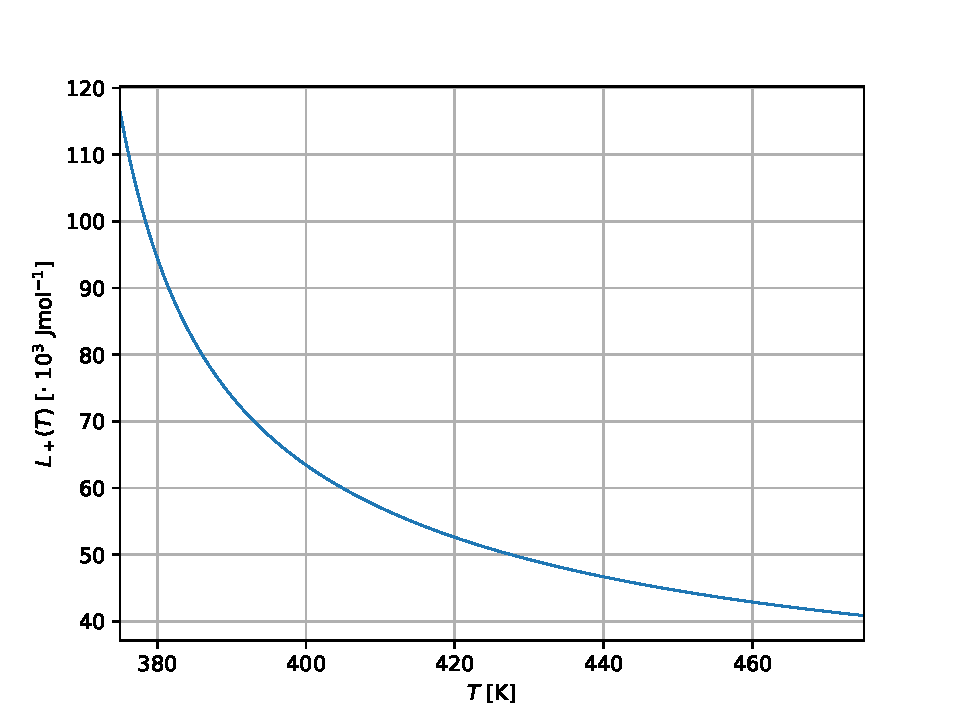
\includegraphics{plot4.pdf}
      \caption{Lösung für die Wärmeenergie $L_2$ bei positivem Wurzelvorzeichen.}
      \label{fig:L_+}
    \end{figure}

    \begin{figure}[H]
      \centering
      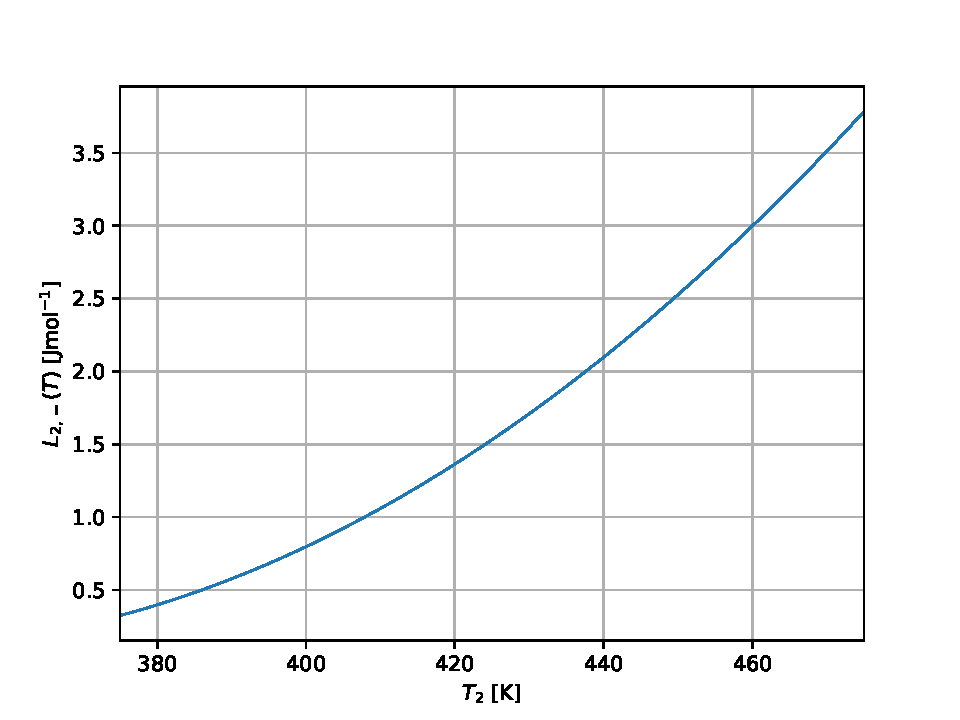
\includegraphics{plot3.pdf}
      \caption{Lösung für die Wärmeenergie $L_2$ bei negativem Wurzelvorzeichen.}
      \label{fig:L_-}
    \end{figure}
    %Siehe \autoref{fig:plot}!
%
%Alte Tabelle: 
    %\begin{table}[H]
    %  \centering
    %  \caption{Gemessener Druck $p$ bei verschiedenen Temperaturen $T$}
    %  \label{tab:Druck_unter_1_bar1}
    %  \begin{tblr}{colspec={c c c c c c}}
    %      \toprule
    %      $T \, \left[\unit{\celsius}\right]$ & $p \, \left[\unit{\milli\bar}\right]$ & $T \, \left[\unit{\celsius}\right]$ & $p \, \left[\unit{\milli\bar}\right]$ & $T \, \left[\unit{\celsius}\right]$ & $p \, \left[\unit{\milli\bar}\right]$\\ 
    %      \midrule
    %      25 \pm 1 & 95 \pm 1   & 51 \pm 1 & 197 \pm 1 & 77 \pm 1 & 438 \pm 1 \\                     
    %      26 \pm 1 & 98 \pm 1   & 52 \pm 1 & 202 \pm 1 & 78 \pm 1 & 453 \pm 1 \\                               
    %      27 \pm 1 & 102 \pm 1  & 53 \pm 1 & 207 \pm 1 & 79 \pm 1 & 471 \pm 1 \\                   
    %      28 \pm 1 & 105 \pm 1  & 54 \pm 1 & 212 \pm 1 & 80 \pm 1 & 487 \pm 1 \\                   
    %      29 \pm 1 & 108 \pm 1  & 55 \pm 1 & 218 \pm 1 & 81 \pm 1 & 507 \pm 1 \\                  
    %      30 \pm 1 & 112 \pm 1  & 56 \pm 1 & 225 \pm 1 & 82 \pm 1 & 528 \pm 1 \\                   
    %      31 \pm 1 & 116 \pm 1  & 57 \pm 1 & 231 \pm 1 & 83 \pm 1 & 547 \pm 1 \\                   
    %      32 \pm 1 & 119 \pm 1  & 58 \pm 1 & 237 \pm 1 & 84 \pm 1 & 578 \pm 1 \\                   
    %      33 \pm 1 & 122 \pm 1  & 59 \pm 1 & 245 \pm 1 & 85 \pm 1 & 592 \pm 1 \\                   
    %      34 \pm 1 & 126 \pm 1  & 60 \pm 1 & 252 \pm 1 & 86 \pm 1 & 612 \pm 1 \\                   
    %      35 \pm 1 & 131 \pm 1  & 61 \pm 1 & 258 \pm 1 & 87 \pm 1 & 635 \pm 1 \\                   
    %      36 \pm 1 & 134 \pm 1  & 62 \pm 1 & 265 \pm 1 & 88 \pm 1 & 656 \pm 1 \\                   
    %      37 \pm 1 & 138 \pm 1  & 63 \pm 1 & 273 \pm 1 & 89 \pm 1 & 678 \pm 1 \\                   
    %      38 \pm 1 & 141 \pm 1  & 64 \pm 1 & 281 \pm 1 & 90 \pm 1 & 700 \pm 1 \\                   
    %      39 \pm 1 & 145 \pm 1  & 65 \pm 1 & 290 \pm 1 & 91 \pm 1 & 724 \pm 1 \\                   
    %      40 \pm 1 & 149 \pm 1  & 66 \pm 1 & 299 \pm 1 & 92 \pm 1 & 753 \pm 1 \\                  
    %      41 \pm 1 & 153 \pm 1  & 67 \pm 1 & 308 \pm 1 & 93 \pm 1 & 775 \pm 1 \\                   
    %      42 \pm 1 & 157 \pm 1  & 68 \pm 1 & 317 \pm 1 & 94 \pm 1 & 809 \pm 1 \\                   
    %      43 \pm 1 & 162 \pm 1  & 69 \pm 1 & 327 \pm 1 & 95 \pm 1 & 835 \pm 1 \\                   
    %      44 \pm 1 & 166 \pm 1  & 70 \pm 1 & 337 \pm 1 & 96 \pm 1 & 867 \pm 1 \\                   
    %      45 \pm 1 & 170 \pm 1  & 71 \pm 1 & 348 \pm 1 & 97 \pm 1 & 899 \pm 1 \\                    
    %      46 \pm 1 & 174 \pm 1  & 72 \pm 1 & 360 \pm 1 & 98 \pm 1 & 938 \pm 1 \\                   
    %      47 \pm 1 & 178 \pm 1  & 73 \pm 1 & 373 \pm 1 & 99 \pm 1 & 989 \pm 1 \\                   
    %      48 \pm 1 & 183 \pm 1  & 74 \pm 1 & 387 \pm 1 & 100 \pm 1 & 999 \pm 1 \\                   
    %      49 \pm 1 & 187 \pm 1  & 75 \pm 1 & 401 \pm 1 & & \\ 
    %      50 \pm 1 & 192 \pm 1  & 76 \pm 1 & 417 \pm 1 & & \\ 
    %               
    %      \bottomrule
    %  \end{tblr}
    %\end{table}